\section{\ac{lora}}
\subsection{Overview}
\ac{lora} is a physical long-range, low-power, communication technology developed and patented by Semtech\footnote{Semtech, USA, https://www.semtech.com/}. It is designed to operate inside either the Sub-1GHz or 2.4GHz unlicensed \ac{ism} bands worldwide. Consequently, under the proviso that local regulatory standards are obeyed (see Section \ref{sec:ISMBandRegulation}), it can be used for wide area deployments without being tied to expensive licensed carriers. Fundamentally, even using its fastest configuration, it is a low-data rate modulation technique. Performance calculations provided are based on Semtech's current Sub-1GHz LoRa transceiver designs (SX1276/77/78/79) \cite{3YP:LORA_SX12}.

Long-range communication can be a challenge in the \ac{ism} bands as the heavy congestion can result in a high physical noise floor. This being the sum of all signals in the band from sources such as the atmosphere or radio devices, excluding that of the signal being monitored. \ac{lora} is one solution to this, it functions using a unique chirp spread spectrum (\ac{css}) modulation technique that can operate below the noise floor. Spread spectrum techniques allow signal-to-noise degradation in a single channel to be compensated for by spreading across other channels. Unlike other \ac{css} techniques that use a fixed chip sequence to carry out spreading, \ac{lora} modulation uses a chirp signal that varies in frequency continuously; this allows the complexity of the receiver design to be greatly reduced and has resulted in a reduced and accessible hardware cost \cite{3YP:LORA_MOD_BASICS}.

The modulation technique means \ac{lora} can boast a far more adaptive and efficient link budget compared to frequency shift keying (FSK) and other modulation types \cite{3YP:LORA_MOD_BASICS}. The link budget being the measure of all gains and losses incurred by a signal passing through the transmitter, the receiver and the propagation channel. This equation in its simplest form is as follows:
\begin{equation}
\label{link_budget}
RX\ Power\ (dB)\ = TX\ Power\ (dB)\ +\ Gains\ (dB)\ -\ Losses\ (dB)
\end{equation}

\subsection{Parameters}
\ac{lora} hardware has many parameters that can be configured to extend range or increase reliability at the expense of air time, data-rate or energy consumption. These are independent from any external hardware and include:
\begin{itemize}
    \item \textbf{Bandwidth (\ac{bw})}: The range of the chirps around the \ac{cf}. Increasing bandwidth increases data-rate but decreases receiver sensitivity \cite{3YP:STUDY_OF_LORA}.
    \item \textbf{Carrier frequency (\ac{cf})}: The centre frequency of chirps. Current hardware targets some sub-range of 137MHz to 1020MHz at a resolution of 61Hz \cite{3YP:LORA_SX12}. 
    \item \textbf{Coding rate (\ac{cr})}: The amount of redundant information encoded in symbols for forward error correction (\ac{fec}); trade-offs can be seen in Table \ref{cr_effect}.
    \item \textbf{Preamble length (\ac{pl})}: The header length of a sent packet used to synchronise transmission. Packet error rate (\ac{per}) has been shown to decrease with an increased \ac{pl} up to a certain threshold \cite{3YP:LORA_PERFORMANCE}. Increasing length can also improve performance of \ac{cad} (see Section \ref{sec:cad}).
    \item \textbf{Spreading factor (\ac{sf})}: The ratio of chip rate to bit rate, where chips per symbol is given as $2^{SF}$. Receiver sensitivity increases in line with spreading factor and is therefore a factor in the link budget \cite{3YP:LORA_SX12}. The trade-offs can be seen in Table \ref{sf_effect}.
    \item \textbf{Transmission power (\ac{tp})}: The radio output power. Equation \ref{link_budget} highlights how an increased \ac{tp} directly increases link budget with the obvious drawback of higher power usage.
\end{itemize}
Figure \ref{lora_transmission_structure} highlights how these parameters affect the structure of a \ac{lora} transmission. The effect on airtime is explained in Section \ref{sec:LoRaTiming}.

\begin{table}
\centering\small
\caption[Effect of \ac{cr}s on \ac{lora} transmissions]{Effect of \ac{cr}s on \ac{lora} transmissions. Recovery performance is defined as the best case percentage of bits that can be lost for a successful receive. \\ Compiled from data in \cite{3YP:LORA_PERFORMANCE}.}
\label{cr_effect}
\begin{tabular}{c|cc}
    \toprule
    \textbf{Coding Rate} & \textbf{Data Overhead} & \textbf{Recovery}  \\
    \midrule\addlinespace
    4/5 & $\times$1.25 & 20\% \\
    4/6 & $\times$1.50 & 33\% \\
    4/7 & $\times$1.75 & 43\% \\
    4/8 & $\times$2.00 & 50\% \\
    \addlinespace\bottomrule
\end{tabular}
\end{table}

\begin{table}
\centering\small
\caption[Effect of \ac{sf} on \ac{lora} transmissions]{Effect of \ac{sf} on \ac{lora} transmissions (\ac{bw}=125KHz). Compiled from data in \cite{3YP:LORA_MOD_BASICS} and \cite{3YP:LORA_PERFORMANCE}.}
\begin{tabular}{c|ccc}
    \toprule
    \makecell{\textbf{\ac{sf}} \\ \textbf{(\ac{lora} Mode)}} & \makecell{\textbf{\ac{sf}} \\ \textbf{(Chirps / Symbol)}} & \makecell{\textbf{Bit Rate} \\ \textbf{(bits / sec)}} & \makecell{\textbf{Demodulation Limit} \\ \textbf{(\ac{snr} dBm)}} \\
    \midrule\addlinespace
    SF7 & 128 & 5469 & -7.5 \\
    SF8 & 256 & 3125 & -10.0 \\
    SF9 & 512 & 1758 & -12.5 \\
    SF10 & 1024 & 977 & -15.0 \\
    SF11 & 2048 & 537 & -17.5 \\
    SF12 & 4096 & 293 & -20.0 \\
    \addlinespace\bottomrule
\end{tabular}
\label{sf_effect}
\end{table}
Selection of these parameters will often be manual, however mechanisms such as \ac{adr} (see Section \ref{sec:lorawanADR}) or ``probing algorithms'', as proposed by \cite{3YP:CHOOSING_LORA_PARAMETERS}, can be used to choose these parameters such that transmission energy is reduced whilst maintaining an adequate throughput and link budget. These methods, due to their overhead, are most suited to static nodes communicating with a gateway.

\begin{figure}[H]
    \centering
   	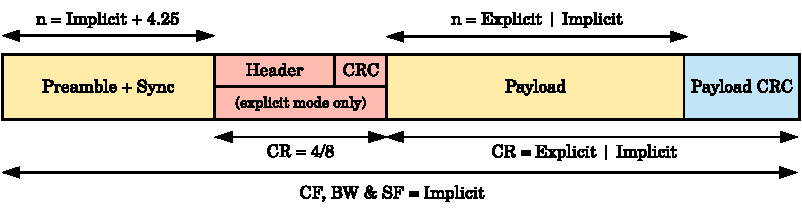
\includegraphics{Figures/lora_transmission.pdf}
    \caption[\ac{lora} transmission packet structure]{
    Structure of a standard \ac{lora} transmission. All transmissions contain a preamble, sync words, and a payload. The header section (in red) is optional but if present, contains information such as the payload length, the payload coding rate, and whether the \ac{crc} is present. If the header is not present this information must be fixed implicitly by the receiver. Parameters that are not in the header are always implicit and must match between transmitter and receiver (i.e. \ac{pl}, \ac{sf}, \ac{bw} and \ac{cf}). Adapted from \cite{3YP:LORA_SX12}.
    }
    \label{lora_transmission_structure}
\end{figure}

\subsection{Considerations}
It should be noted that \ac{lora} radios, like all current consumer radios, are half-duplex, meaning that they are unable to receive during transmission; this can result in missed receives. Consideration should also be given for the differing technology in transceivers and gateways. A gateway contains a \ac{lora} concentrator block, allowing demodulation of up to eight signals concurrently provided they use unique spreading factors \cite{3YP:LORA_SX1301}. A transceiver can only demodulate one signal at a time \cite{3YP:LORA_SX12}. Collisions may occur in the presence of conflicting signals, resulting in failed receives; the conditions of this occurrence are assessed further in Section \ref{sec:RadioCollisions}. Most \ac{lora} applications consist of many sensor nodes infrequently sending data to a single gateway with very little downlink; this means collisions and missed receives are rare. Unfortunately, in a mesh-like point-to-point network, these events are a very real possibility. High data-rate wireless communications, such as Wi-Fi, will often use carrier-sense multiple access (CSMA) mechanisms to allow for full-duplex emulation, but with LoRa this can lead to a waste of precious available airtime. Nonetheless, implementations using LoRa's \ac{cad} have been attempted with promising results for a single point-to-point transmission \cite{3YP:LORA_CSMA}. Though gateways are clearly more powerful than transceivers, their cost and power usage make them hard to deploy on scale. That being said, Pycom's\footnote{Pycom, UK,  https://pycom.io/} newly released Pygate gateway is a fraction of the cost of existing implementations and may be feasible for an ad-hoc scenario.
\subsection{Channel Activity Detection (\ac{cad})}\label{sec:cad}
Carrier-sensing is a helpful mechanism for radios to check whether a channel is busy or idle. Usually, this is achieved by checking the power present in the channel using the received signal strength indicator (\ac{rssi}). This is a very unreliable method for \ac{lora} because the \ac{rssi} includes channel noise, and \ac{lora} signals can operate below the noise floor. For this reason, \ac{lora} radios offer a specialised \ac{cad} method, which searches the channel for a single \ac{lora} packet preamble symbol. \ac{cad} is at least 97\% reliable in the presence of preamble with false positives occuring just 0.1\% of the time \cite{3YP:LORA_FOR_IOT}. It has been shown that \ac{cad} can in fact detect non-preamble symbols when there is high signal strength, although this ability quickly becomes unreliable in a real world scenario \cite{3YP:LORA_CSMA}.

\subsection{Signal Orthogonality}
The manner of \ac{lora}'s modulation allows multiple signals to co-exist in the same channel provided they have a different chirp rate ($C_R$), where $C_R = BW \times S_R$. $S_R$ (symbol rate) is calculated as the chip rate, which is directly defined by the \ac{bw}, divided by the number of chips per symbol, $S_R=\frac{BW}{2^{SF}}$. This clearly demonstrates that for a single bandwidth, all \ac{sf}s must be orthogonal to one another. However, in the case that different \ac{bw}s are used, different \ac{sf}s may have the same chirp rate and could interfere; this is demonstrated in Figure \ref{fig:orthogonality}.

\begin{figure}[H]
    \centering
   	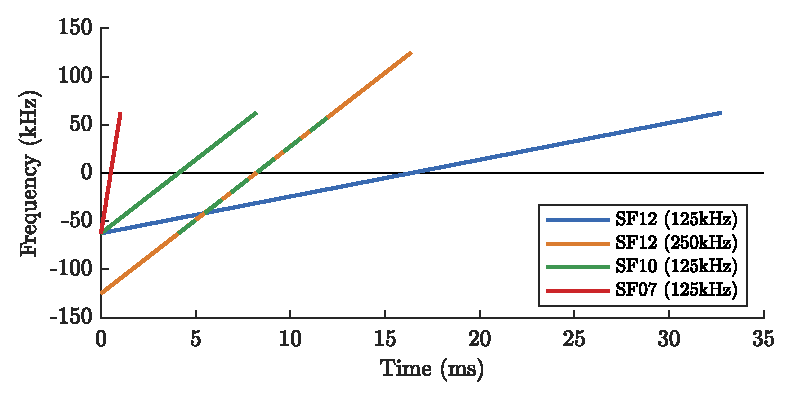
\includegraphics{Figures/sf_orthogonality_plot.eps}
    \caption[Signal chirp rate orthogonality]{
    Demonstration of signal orthogonality for different \ac{sf}s. The SF10 (125kHz) chirp is duplicated and shifted to overlap with the  SF12 (250kHz) chirp to highlight that they have the same chirp rate and are therefore not orthogonal.
    }
    \label{fig:orthogonality}
\end{figure}
%Symbol duration is the inverse of the symbol rate, defined in \ref{cr_effect}

